\documentclass{beamer}
\usepackage{amsthm}
\usepackage{amsmath}
\usepackage{amsfonts}
\usepackage{amssymb}
\usepackage{epic}
\usepackage{graphicx}
\usepackage{epstopdf}
\usepackage{multirow}
\usetheme{JuanLesPins}
\usecolortheme{default}
\usepackage{multicol}



\newtheorem{question}{Question}[section]

\title{Analysis of geographical patterns in weather-related flight delays}


\author{Mathew Edwards, Nandhita Narendra Babu, Wanli Zhang}

\date{\today}

\begin{document}

\begin{frame}
\titlepage
\end{frame}

\begin{frame}{\contentsname}
\tableofcontents
\end{frame}

\section{Introduction}

\begin{frame}
\frametitle{Data Information}
\begin{itemize}
\item Airline on time data from the Bureau of Transportation Statistics for all US States

\item[]

\item Weather-related flight delays data from June 2003 to December 2013
\end{itemize}
\end{frame}


\begin{frame}
\frametitle{Question of Interest}
Are there geographical patterns in weather-related flight delays, and do these change over time?
\end{frame}


%-------------------------------------------------------------------------------%



\section{Population-based Analysis}
\begin{frame}
\frametitle{Assumptions} 
\begin{itemize}
\item NA $\rightarrow$ No Delay

\item For Proportion
\begin{itemize}
\item Weather delay value greater than 0 $\rightarrow$ 'Delayed' regardless of severity 
\item Denominator $\rightarrow$ count of all flights including NA
\end{itemize}

\item Weather within a month is 'reasonably consistent'

\item Defined regions using National Oceanic and Atmospheric Administration (NOAA) map
\begin{itemize}
\item Added Alaska and Hawaii as their own region
\item Lumped unlinked airports into an 'Other' region
\end{itemize}

\item Weather is similar in climate regions

\item Analysis done on origin airport. Assumes delay on origin side.

\end{itemize}
\end{frame}





\begin{frame}
\frametitle{NOAA Map of Regions}
\begin{center}
  \scalebox{0.57}{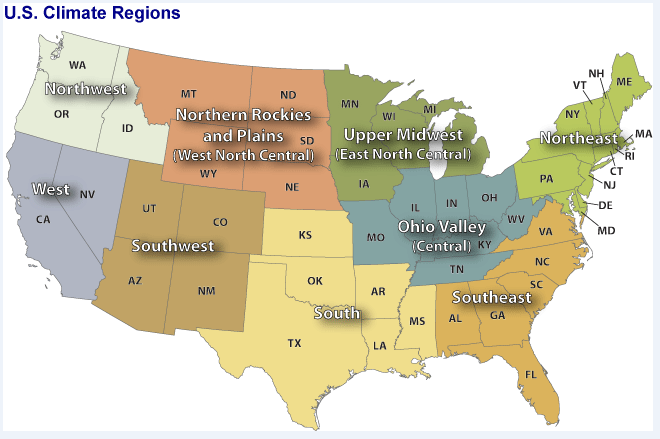
\includegraphics{../Maps/NOAA-map.png}}
\end{center}
\end{frame}






\begin{frame}
\frametitle{Population-based Results}
\begin{itemize}
\item Aggregate to monthly basis

\item Higher percentages of delayed flights are in winter

\item Highest winter proportions are in Central region
\begin{itemize}
\item Chicago: Major hub plus cold winters
\end{itemize}

\item No month/region exceeds $4\%$ in the proportion of delayed flights

\item Bump in Jun, Jul and August for the South, Southeast, Northeast and Upper Midwest
\begin{itemize}
\item Tornado season?
\end{itemize}

\item South is consistently above $1\%$ across all months

\end{itemize}
\end{frame}




\begin{frame}
\frametitle{Proportion of Weather Delayed Flights, by Month}
\begin{center}
  \scalebox{0.45}{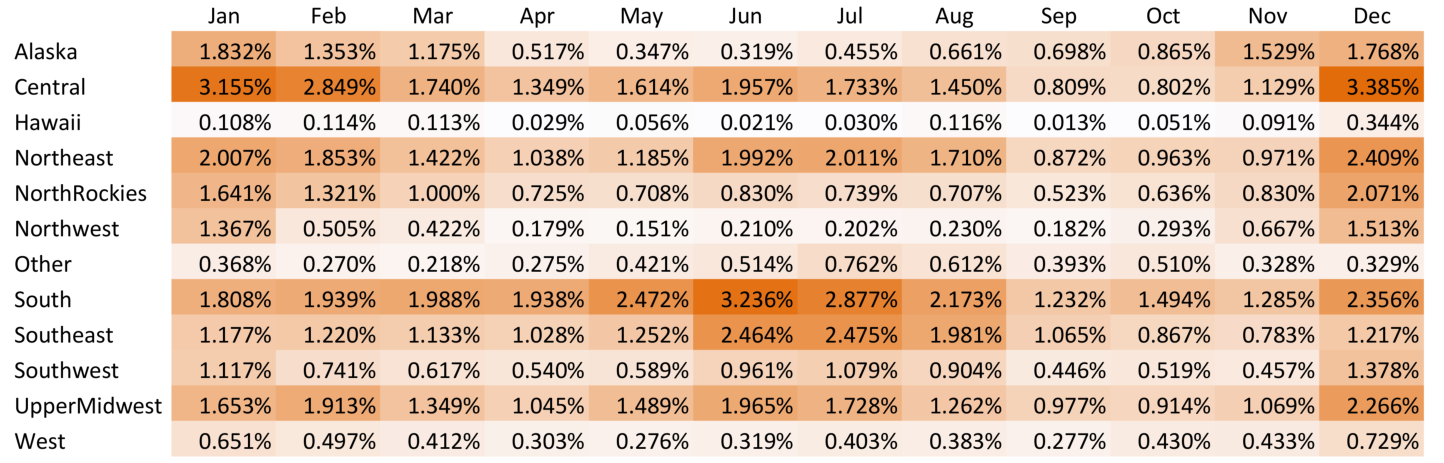
\includegraphics{../Images/PopnSummary_USE.pdf}}
\end{center}
\end{frame}



\begin{frame}
\frametitle{Population-based Results}
\begin{itemize}
\item Across all years

\item[]

\item Northern Rockies show greatest fluctuation over the years

\item[]

\item Consistently low percentage of delayed flights in northeastern area

\item[]

\item Northern Rockies alone:
\begin{itemize}
\item No obvious seasonal patterns
\item Gradual change of mean level over the years
\end{itemize}

\end{itemize}
\end{frame}



\begin{frame}
\frametitle{All Regions}
\begin{center}
  \scalebox{0.52}{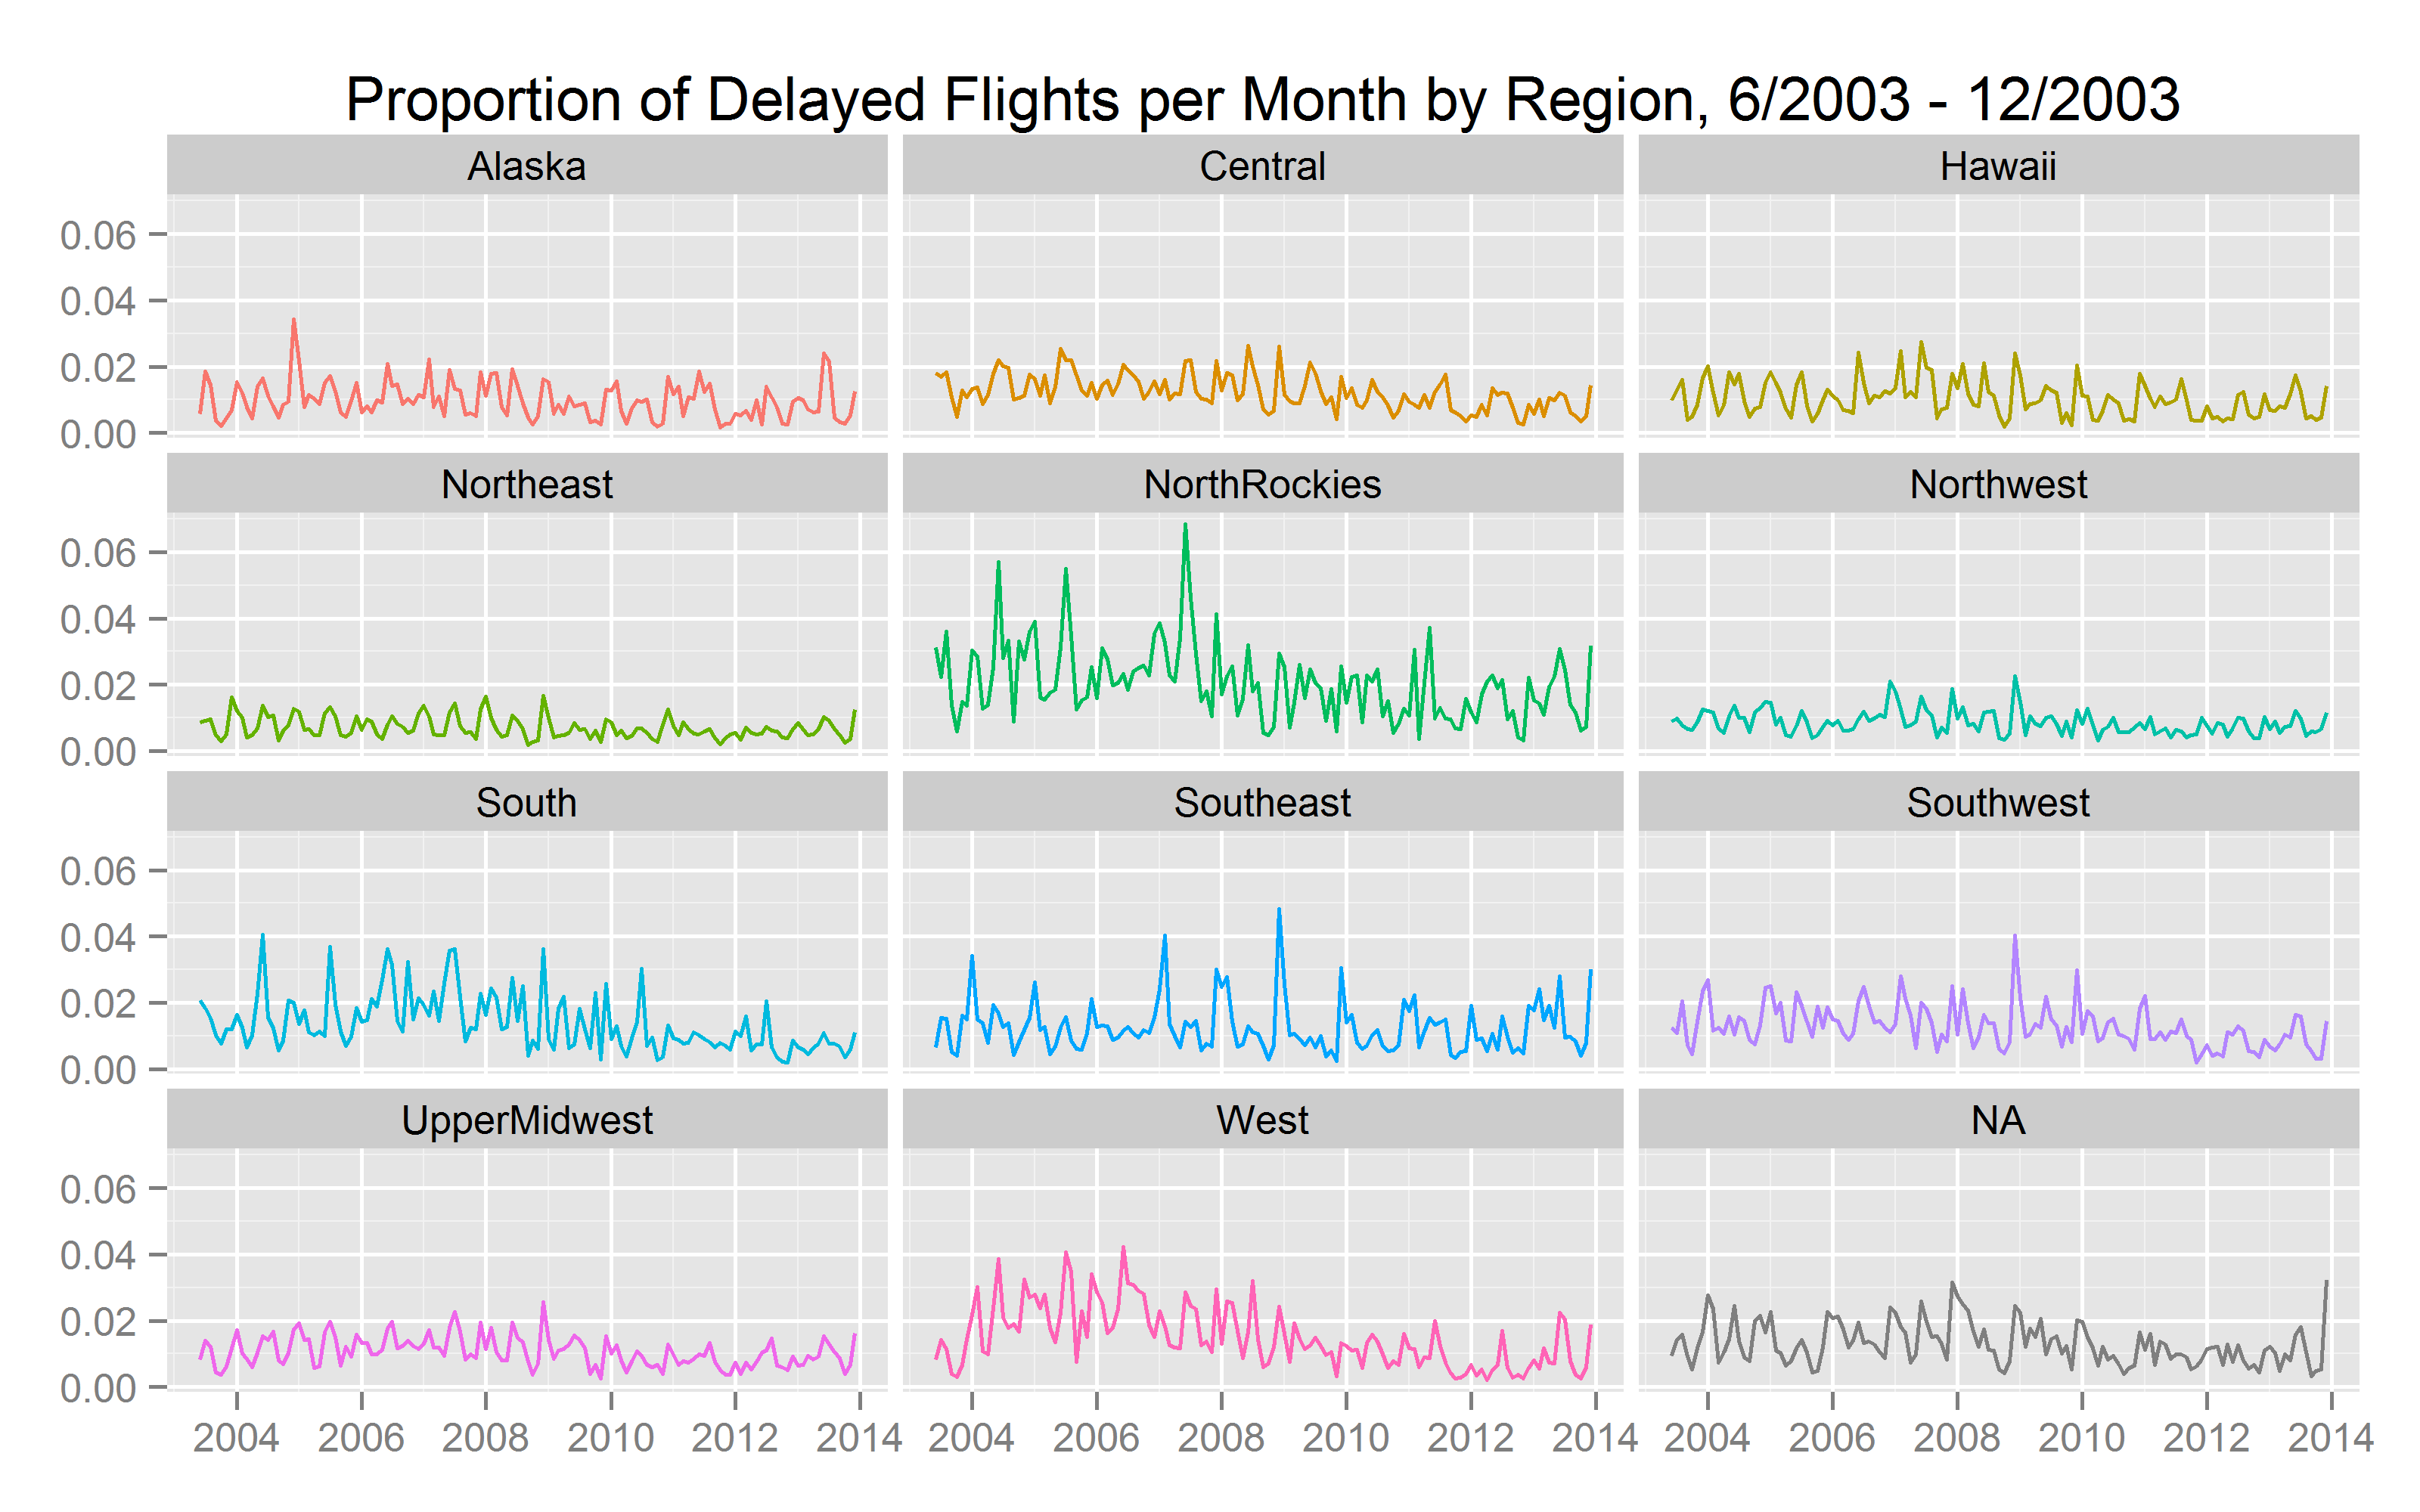
\includegraphics{../Images/popn_prop.png}}
\end{center}
\end{frame}



\begin{frame}
\frametitle{Northern Rockies}
\begin{center}
  \scalebox{0.45}{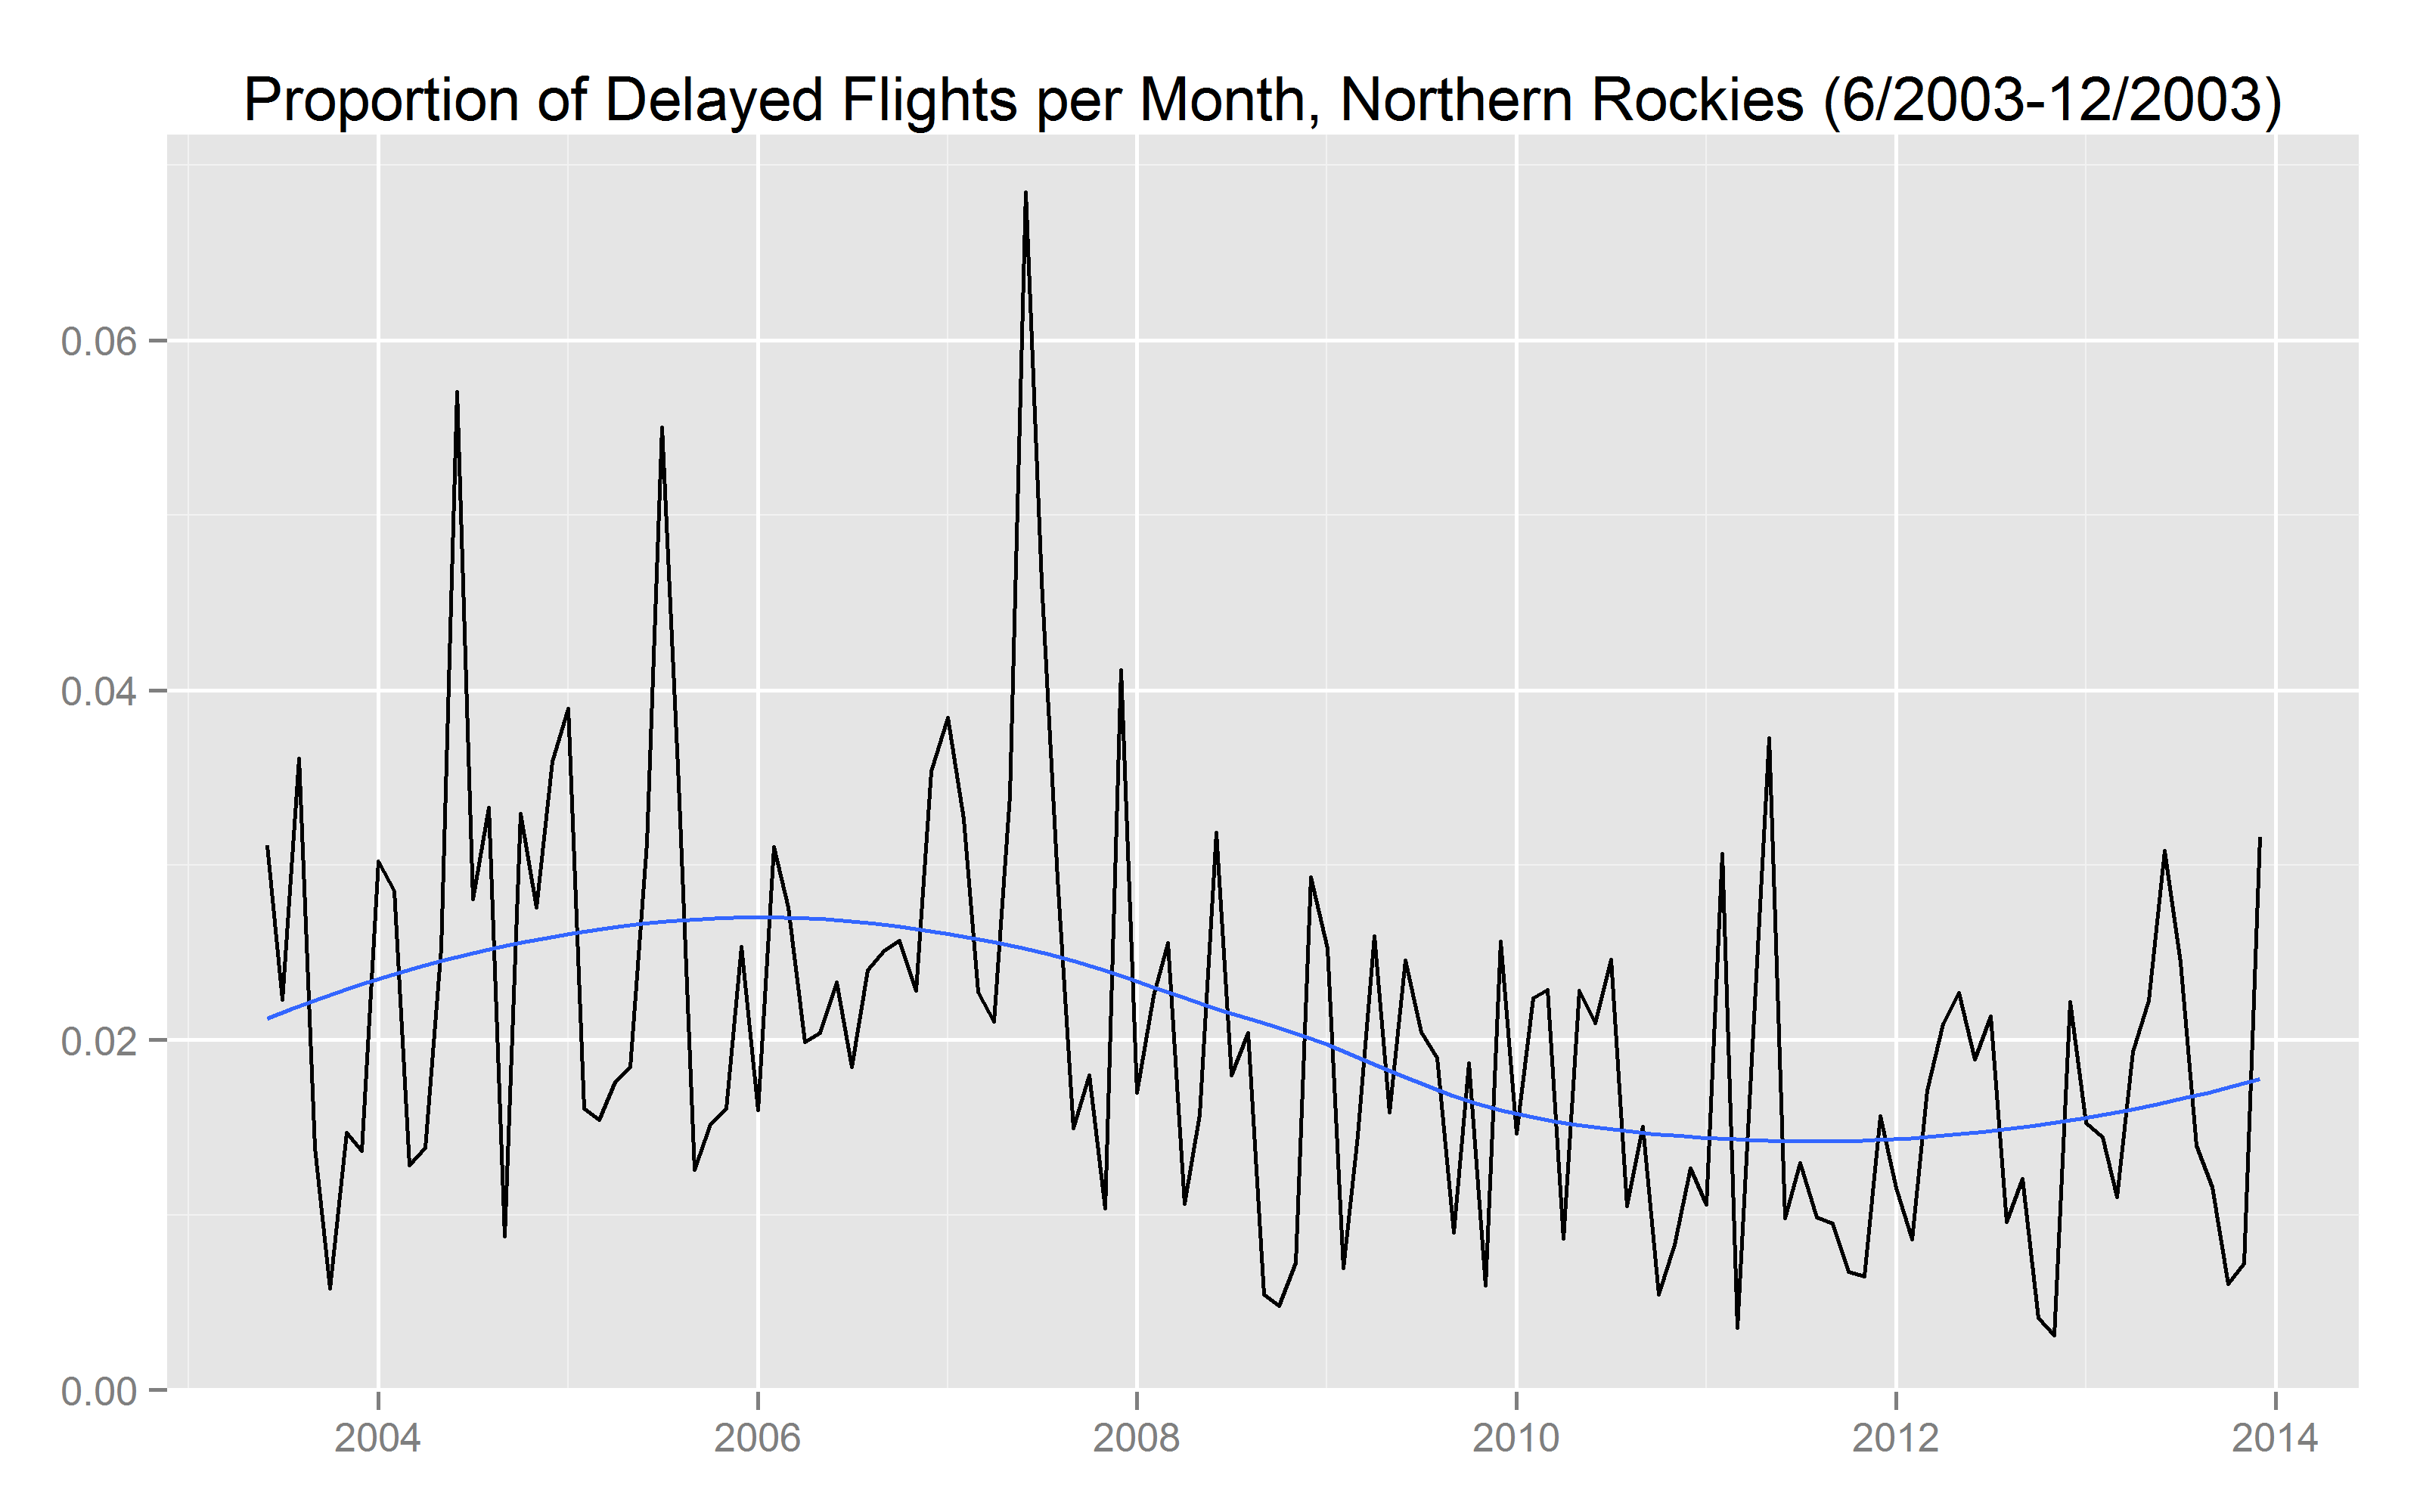
\includegraphics{../Images/popn_prop_northrockies.png}}
\end{center}
\end{frame}





%---------------------------------------------------------------------------------%


                        %---- Sample-based analysis ----%


\section{Sampling Based Analysis}
\begin{frame}
\frametitle{Assumptions}
\begin{center}
Same as that of Population Based Analysis 
\end{center}
\end{frame}




\begin{frame}
\frametitle{Sampling Technique}
\begin{itemize}
\item Strata $\rightarrow$ Single region for single month

\item[]

\item Number of flights per month ranging from an average of 3,000 in Alaska to an average of 115,000 in the Southwest

\item[]

\item Proportional sampling $\rightarrow$ sampled approximately 2.5\% of the flights in each
stratum
\end{itemize} 
\end{frame}





\begin{frame}
\frametitle{Sample-based Results}
\begin{itemize}

\item Very similar to the population results

\item[]

\item Heat map of monthly proportions show the same pattern
\begin{itemize}
\item Nothing over 4\%
\item Same bump in the summer in the south
\end{itemize}

\item[]

\item Zero proportion in some strata, with very low population proportions

\item[]

\item Standard errors all below 0.5\%, and generally below 0.25\%


\end{itemize}
\end{frame}





\begin{frame}
\frametitle{Proportion of Weather Delayed Flights, by Month}
\begin{center}
  \scalebox{0.45}{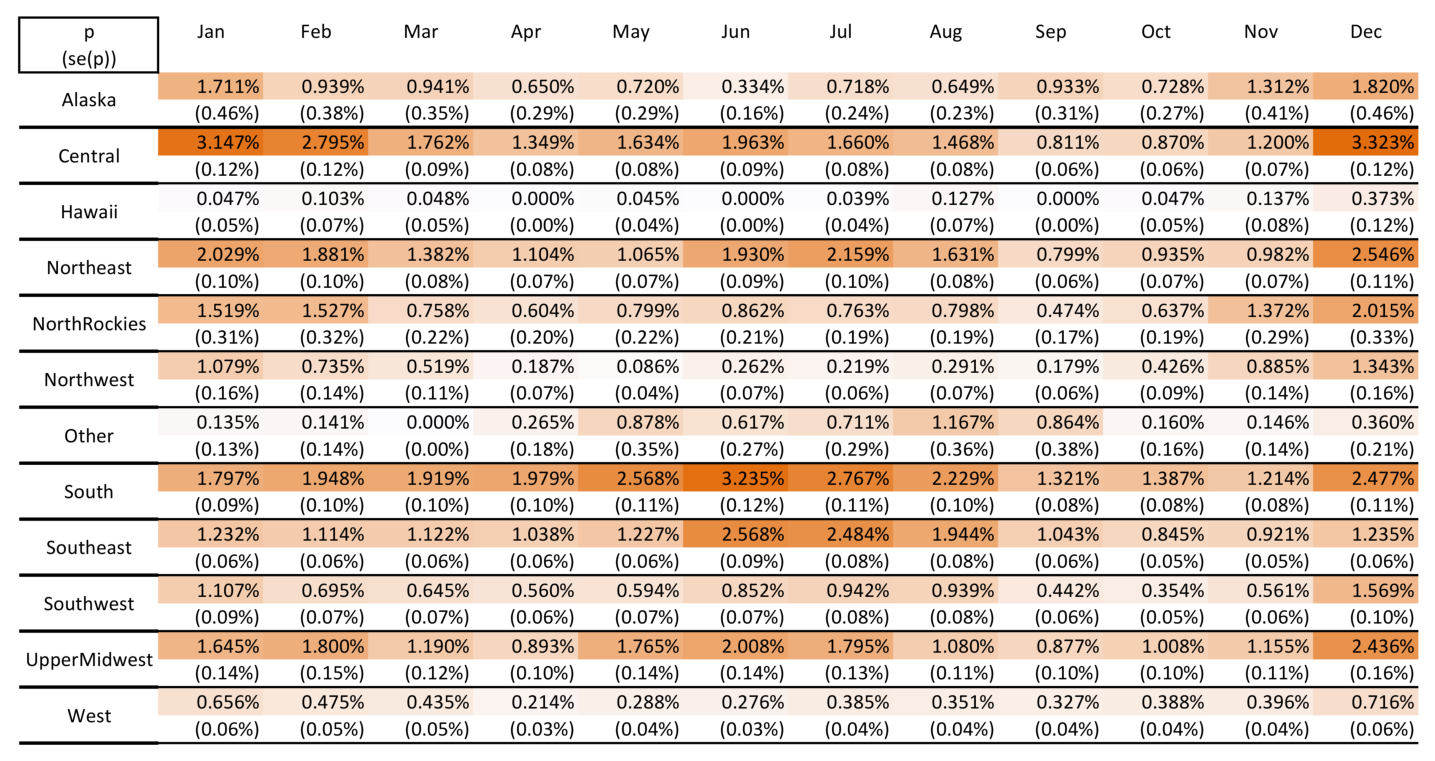
\includegraphics{../Images/SampSumm_USE.pdf}}
\end{center}
\end{frame}




\begin{frame}
\frametitle{Sample-based Analysis}
\begin{itemize}
\item Proportions with point-wise confidence intervals

\item[]

\item Regions Alaska, Hawaii and Other have greater margins of error
\begin{itemize}
\item Small sample sizes
\end{itemize}

\item[]

\item No apparent trend over the years for most regions, except for the South

\item[]

\item South alone:
\begin{itemize}
\item No obvious seasonal patterns
\item Bump at the end of 2006/beginning of 2007
\end{itemize}

\end{itemize}
\end{frame}




\begin{frame}
\frametitle{All Regions}
\begin{center}
  \scalebox{0.52}{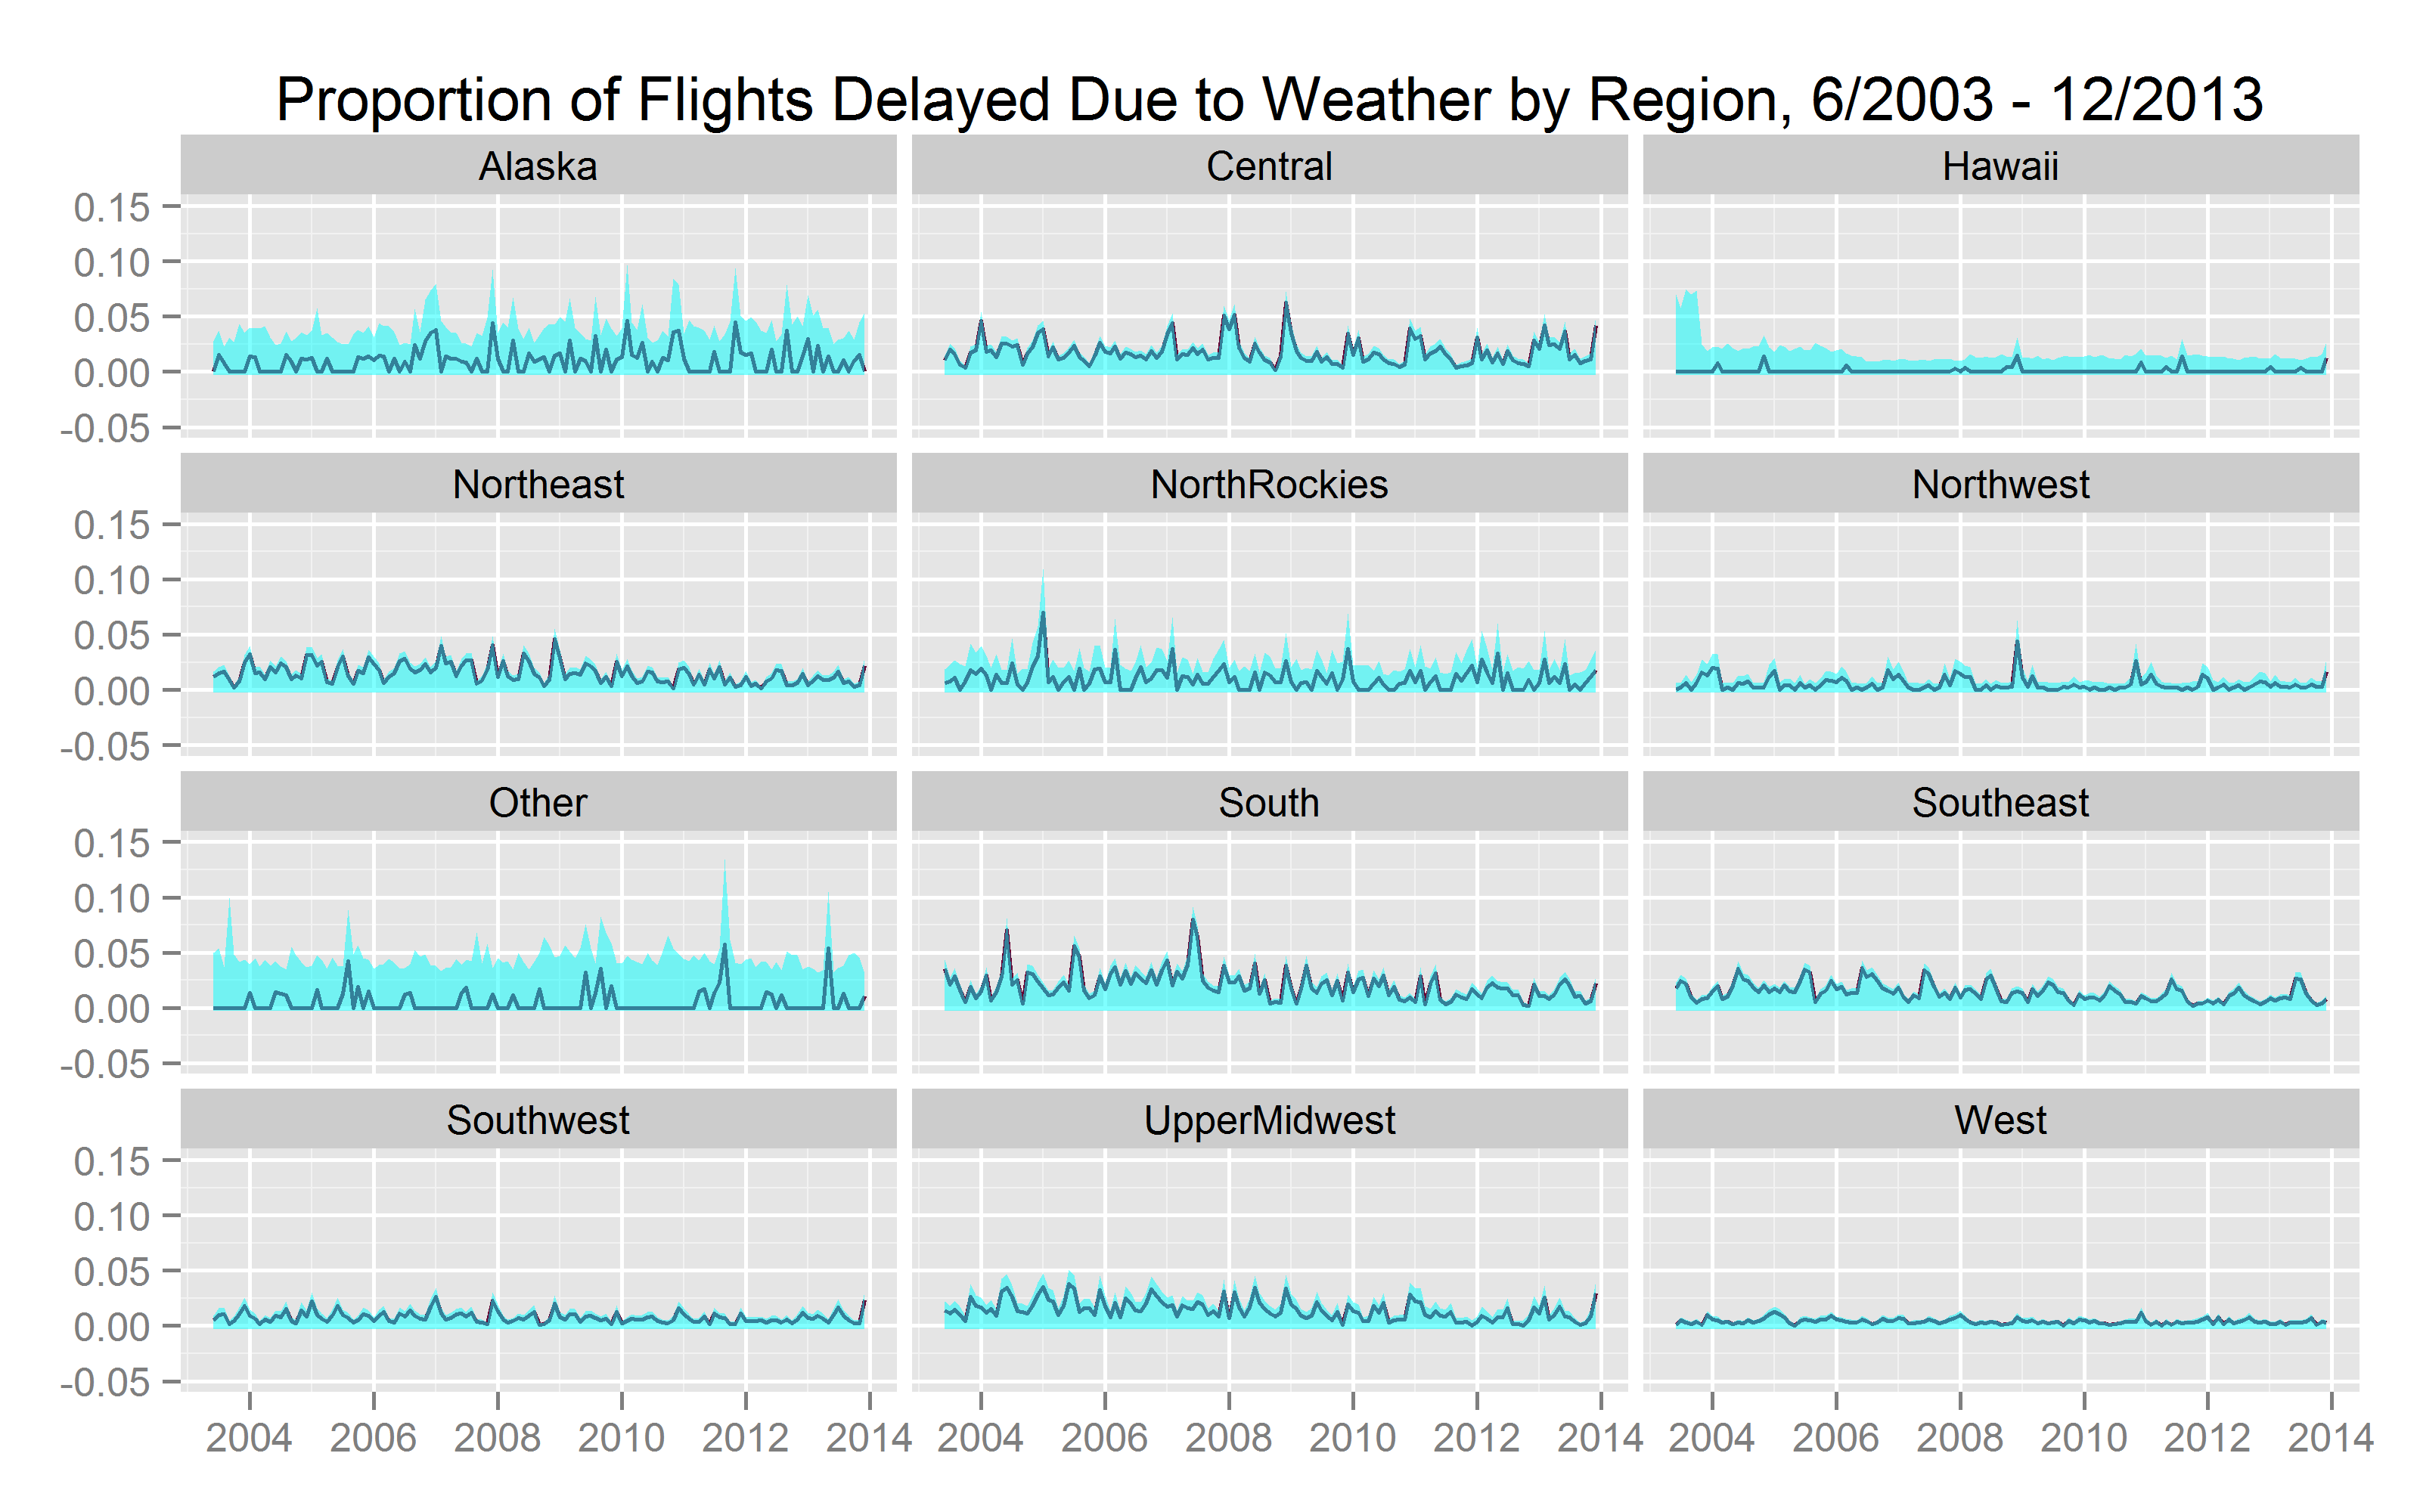
\includegraphics{../Images/samp_prop.png}}
\end{center}
\end{frame}



\begin{frame}
\frametitle{Southern Area}
\begin{center}
  \scalebox{0.52}{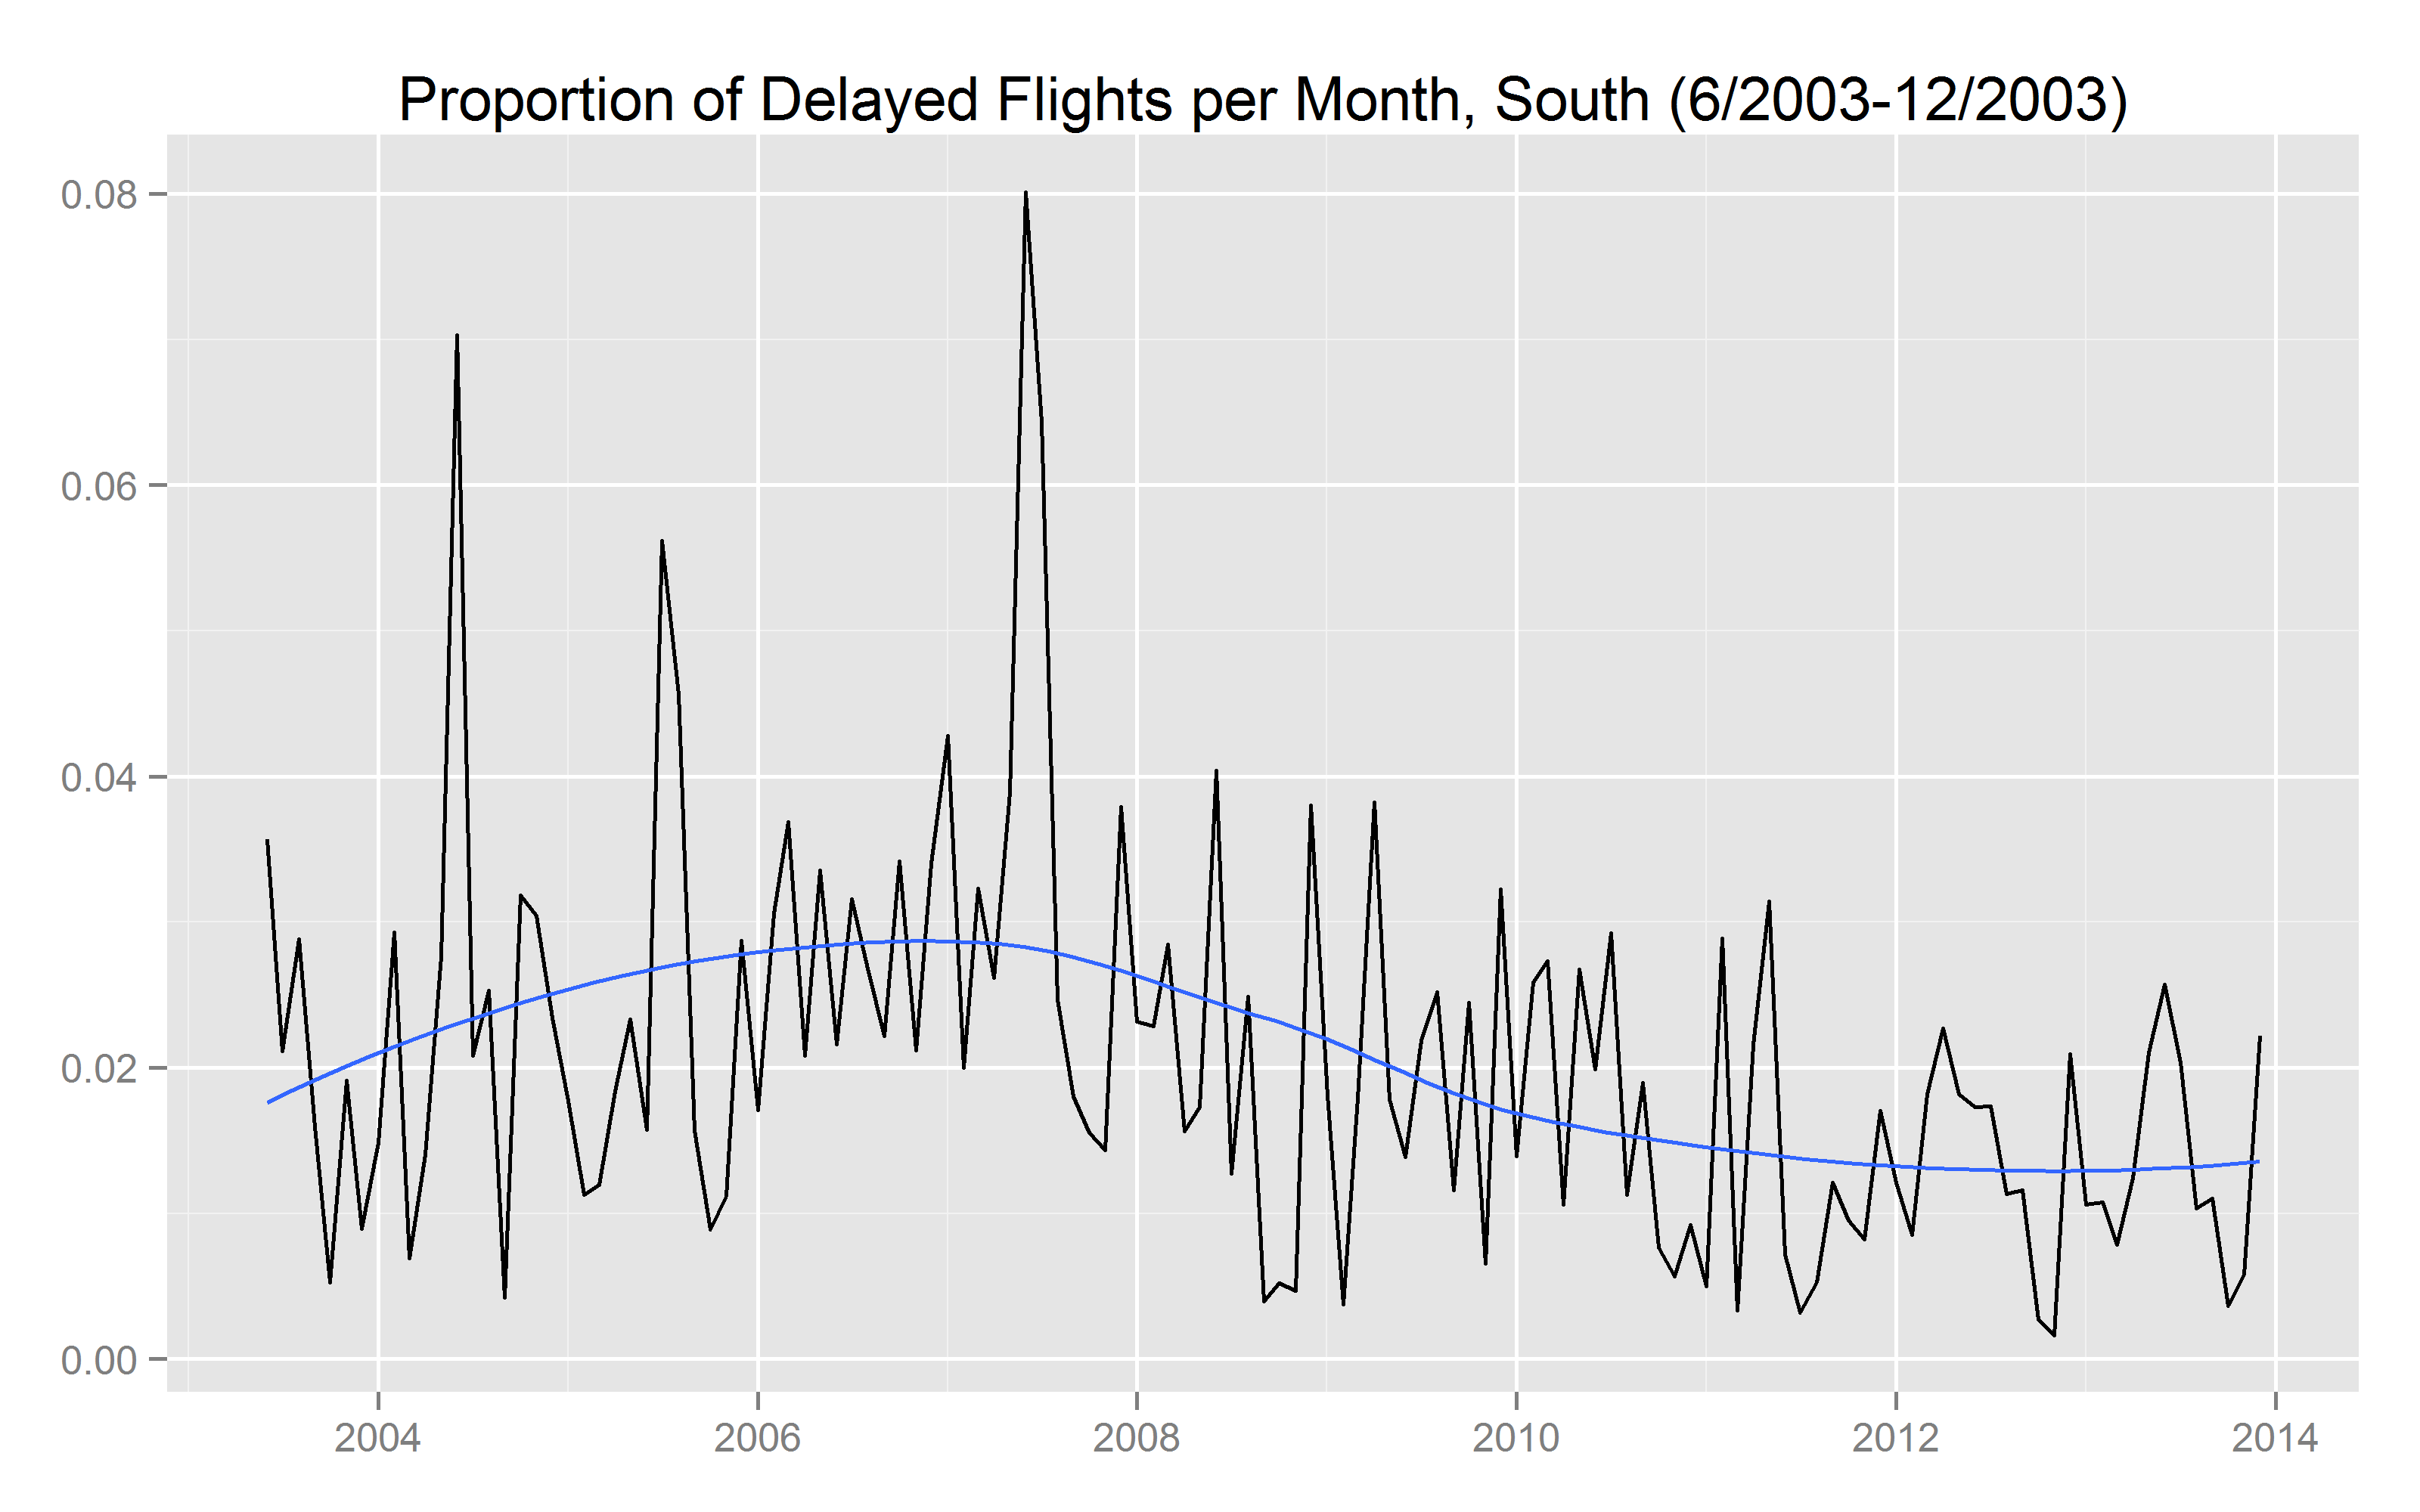
\includegraphics{../Images/samp_prop_south.png}}
\end{center}
\end{frame}
















%----------------------------------------------------------------------------------%



                              %---- Discussion ----%


\section{Discussion, Obstacles and Solutions}
\begin{frame}
\frametitle{Discussion}

\begin{itemize}
\item \textbf{Expecting}: seasonal differences (more delays in winter)

\item[]

\item \textbf{Not expecting}: large amount of summer delays, especially in South and Southeast

\item[]

\item Observed regional differences in amount of delays

\item[]

\item No significant shift in regional differences over time

\end{itemize}
\end{frame}





\begin{frame}
\frametitle{Population and Sample Monthly Proportions}
\begin{center}
  \scalebox{0.34}{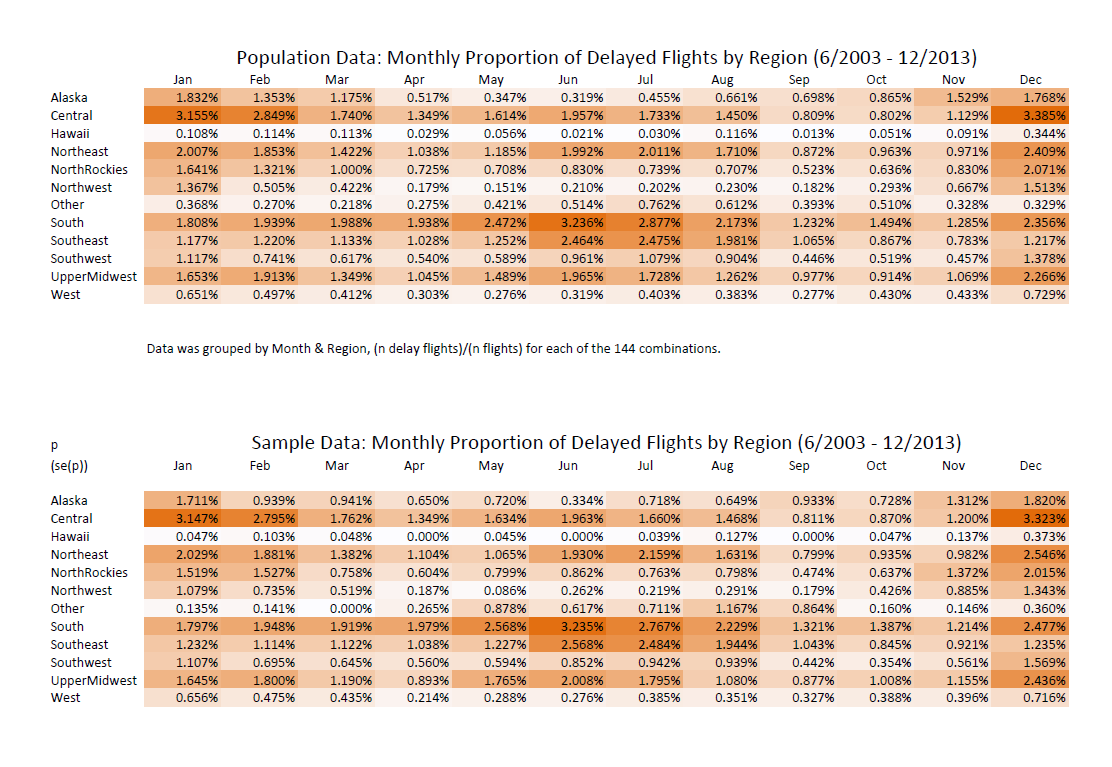
\includegraphics{../Images/ComparePopnandSamp.png}}
\end{center}
\end{frame}








\begin{frame}
\frametitle{Obstacles and Solutions}
\begin{itemize}

\item[]

\item Defining regions $\&$ assigning regions to flights
\begin{itemize}
\item \texttt{left\_join} of DPLYR was very helpful
\item Saved the IATA, State and Region for all airports in a .csv file for easy use
\end{itemize}

\item[]

\item Five IATA codes in the data not documented in the Data Expo .csv file
\begin{itemize}
\item Googled it!
\end{itemize}

\item[]

\end{itemize}
\end{frame}


\begin{frame}
\frametitle{Obstacles and Solutions}
\begin{itemize}

\item[]

\item Figuring out how to sample by our strata (region/month/year)


\begin{itemize}
\item Define list of vectors:
%\texttt{  region.df <- tbl\_df(read.csv(``data/iata_by_region.csv'', header\=T, stringsAsFactors\=F))}


\texttt{ak.list <- [All Alaska Airport Codes] }\\
\texttt{c.list  <- [All Central Airport Codes]}\\
\texttt{\ldots}\\
\texttt{r.list <- list(ak.list, c.list,\ldots)}
\item[]

\item Within loop, assign one vector from list to a variable:\\
\texttt{o.list = r.list[[k]]}\\

\item[]
\item Within filter, use \texttt{\%in\%} statement and list variable:\\
\texttt{filter(\ldots,origin \%in\% o.list,\ldots)}\\


\end{itemize}



\item[]

\end{itemize}
\end{frame}


\begin{frame}
\frametitle{Obstacles and Solutions}
\begin{itemize}

\item[]

\item Confidence intervals for zero proportions
\begin{itemize}
\item Rule of Three: 3/$n_h$ gives upper bound of $95\%$ CI
\end{itemize}

\item[]

\item "Other" region: military bases and protectorates, not geographically consistent
\begin{itemize}
\item Included in summary but no conclusions drawn from it
\end{itemize}

\item[]

\end{itemize}
\end{frame}




















\end{document}